% ****** Start of file apssamp.tex ******
%
%   This file is part of the APS files in the REVTeX 4.1 distribution.
%   Version 4.1r of REVTeX, August 2010
%
%   Copyright (c) 2009, 2010 The American Physical Society.
%
%   See the REVTeX 4 README file for restrictions and more information.
%
% TeX'ing this file requires that you have AMS-LaTeX 2.0 installed
% as well as the rest of the prerequisites for REVTeX 4.1
%
% See the REVTeX 4 README file
% It also requires running BibTeX. The commands are as follows:
%
%  1)  latex apssamp.tex
%  2)  bibtex apssamp
%  3)  latex apssamp.tex
%  4)  latex apssamp.tex
%
\documentclass[%
 reprint,
%superscriptaddress,
%groupedaddress,
%unsortedaddress,
%runinaddress,
%frontmatterverbose, 
%preprint,
%showpacs,preprintnumbers,
%nofootinbib,
%nobibnotes,
%bibnotes,
 amsmath,amssymb,
 aps,
%pra,
%prb,
%rmp,
%prstab,
%prstper,
%floatfix,
]{revtex4-1}

\usepackage{graphicx}% Include figure files
\usepackage{dcolumn}% Align table columns on decimal point
\usepackage{bm}% bold math
%\usepackage{hyperref}% add hypertext capabilities
%\usepackage[mathlines]{lineno}% Enable numbering of text and display math
%\linenumbers\relax % Commence numbering lines

%\usepackage[showframe,%Uncomment any one of the following lines to test 
%%scale=0.7, marginratio={1:1, 2:3}, ignoreall,% default settings
%%text={7in,10in},centering,
%%margin=1.5in,
%%total={6.5in,8.75in}, top=1.2in, left=0.9in, includefoot,
%%height=10in,a5paper,hmargin={3cm,0.8in},
%]{geometry}

\begin{document}

\preprint{APS/123-QED}

\title{Osciloscopio}% Force line breaks with \\
\thanks{A footnote to the article title}%

\author{Ann Author}
 \altaffiliation[Also at ]{Departamento de Física, Universidad de los Andes}%Lines break automatically or can be forced with \\
\author{Sergio Iv\'an Rey}%
 \email{si.rey1826@uniandes.edu.co}
\affiliation{%
 Departamento de Física, Universidad de los Andes
}%

\date{13/8/2015}% It is always \today, today,
             %  but any date may be explicitly specified

\begin{abstract}
Durante la presente práctica se estudiaron los fen\'omenos ondulatororios en circuitos RC, RLC y en osciladores acoplados. En una primera instancia se determin\'o experimentalmente el tiempo de caracter\'istico de carga y descarga de un condensador, donde se encontraron valores muy cercanos a los valores te\'oricos, sin embargo al cambiar de dispositivos se encontraron errores de m\'as de un 50\% lo que lleva a pensar que los \'ultimos dispositivos usados estaban en mal estado. En segunda instancia, se construy\'o un circuito RLC en serie donde, por dos m\'etodos diferentes se determin\'o la frecuencia natural del sistema junto con su tiempo caracter\'istico de carga y descarga. Los valores requirieron de segundas mediciones pero se encuentran dentro de lo esperado.
\end{abstract}


\keywords{Suggested keywords}%Use showkeys class option if keyword
                              %display desired
\maketitle

%\tableofcontents

\section{\label{sec:level1}Introducci\'on}

Las resistencias, capacitancias e inductancias son de los componentes m\'as fundamentales de los circuitos electr\'onicos. Su comportamiento puede ser cuantificado con gran exactitud y por esta raz\'on sirven para estudiar diversos sistemas que van desde sistemas no oscilatorios hasta sistemas de oscilaciones forzadas y amortiguadas. Las diversas aplicaciones de los circuitos RC, RL, LC, RLC, etc. van desde transformadores AC a DC, filtros de señales, hasta generadores simples de voltaje. Estos circuitos son los componentes primordiales de elementos cotidianos como las buj\'ias, los flashes de c\'amaras fotogr\'aficas, etc.\\

En primera instancia, en este laboratorio nos interesamos en estudiar el proceso de carga y descarga de un capacitor en un circuito RC en serie bajo una diferencia de potencial constante ($V_f$). Si se obtiene la ecuación diferencial para la carga del capacitor en estos sistemas, es sencillo demostrar que las funciones de voltaje sobre el capacitor para el sistema de carga ($V_c$) y descarga ($V_d$) son respectivamente:\\

\begin{equation}
Vc(t) = V_f(1-e^{-t/{RC}})
\end{equation}
\begin{equation}
Vd(t) = V_fe^{-t/{RC}}
\end{equation}

En estas ecuaciones, $\tau = RC$ es una constante fundamental que indica qu\'e tan r\'apido se carga o descarga el capacitor. En el caso del proceso de descarga, esta constante indica en cu\'anto tiempo el capacitor llega a un factor de $e^{-1} \approx 37\% $ de su valor inicial. \\

En segunda instancia, para caracterizar un sistema oscilatorio forzado y amortiguado con el osciloscopio, nos propusimos estudiar un circuito RLC en serie. Para este tipo de circuitos, la ecuaci\'on diferencial que caracteriza la carga almacenada en el capacitor es lineal de segundo orden. De forma general, la ecuación diferencial este tipo de sistemas es de la forma:\\

\begin{equation}
\frac{d^2q}{dt^2} + \gamma\frac{dq}{dt} + \omega_0^2q = \frac{F_0}{m}e^{i\omega t}
\end{equation}

Aqu\'i $\omega$ es la frecuencia de forzamiento de la fuente y $F_0$ su amplitud. El par\'ametro $m$ ser\'ia la masa en un sistema mec\'anico. $\omega_0$ es la frecuencia natural del sistema. El par\'ametro $\gamma$ hace referencia a la perdida de energ\'ia del sistema, por fricci\'on en sistemas mec\'anicos, y por resistencia en los electr\'onicos. Estos dos \'ultimos par\'ametros determinan la resonancia del sistema respecto a la fuente de forzamiento, e incluso determinan si la ecuaci\'on diferencial acepta o no soluciones oscilatorias en el caso en que no haya forzamiento ($\omega = 0$).\\

Sin mucho esfuerzo, analizando el circuito RLC en s\'i, es posible deducir que $m \equiv L$, $F_0 \equiv V_f$ y que los valores de los par\'ametros de frecuencia y fricci\'on están dados por:\\

\begin{equation}
\omega_0 = \frac{1}{\sqrt{LC}}
\end{equation}
\begin{equation}
\gamma = R/L
\end{equation}

Si hay la fuente es una onda sinusoidal, es decir, si hay forzamiento, la ecuaci\'on diferencial solo aceptar\'a soluciones de tipo sinusoidal, con frecuencia igual a la de forzamiento ($q(t) = A*e^{i\omega + \delta}$) . En este caso, lo importante es analizar la amplitud de las soliciones en t\'erminos de la frecuencia de forzamiento. Si insertamos la soluci\'on propuesta en la ecuaci\'on diferencial, obtenemos una expresi\'on para la amplitud del sistema en t\'ermonos de la frecuencia de forzamiento:

\begin{equation}
A(\omega) = \frac{V_f/L}{\sqrt{(\omega^2 - \omega_0^2)^2 + (\gamma\omega)^2}}
\label{equation:amplitud}
\end{equation}

Derivando esta expresi\'on, se puede encontrar la frecuencia de forzamiento ($\omega_m$) que produce el m\'aximo de amplitud en el sistema. \'Esta frecuencia estar\'a dada por:\\

\begin{equation}
\omega = \sqrt{\omega_0^2 - \frac{\gamma^2}{2} }
\end{equation}

De la misma manera es sencillo demostrar que el ancho de la curva de resonancia, es decir, la distancia entre los dos valores de frecuencia que producen la mitad de la amplitud m\'axima, est\'a dado por:\\

\begin{equation}
\Delta\omega = \frac{1}{\tau} = \frac{1}{\gamma} = \frac{L}{R}
\end{equation}

En tercera instancia, para analizar un sistema no forzado y amortiguado, tomamos el mismo circuito RLC, esta vez, bajo una fuente directa. En este caso, si se tiene una resistencia lo suficientemente pequeña, la ecuaci\'on diferencial admitir\'a soluciones oscilatorias. En dicho caso, la solución a la ecuaci\'on diferencial (3), con $\omega = 0$  es una onda con la frecuencia $\omega_a = \sqrt{\omega_0^2 -\frac{\gamma^2}{4}}$ , con amplitud modulada por una exponencial determinada por la resistencia. Esta soluci\'on se presenta de la siguiente manera:\\

\begin{equation}
V(t) = V_0 e^{\frac{-\gamma t}{2}}\cos(\omega_a t + \delta)
\end{equation}






\section{\label{sec:level1}Montaje experimental}



\section{\label{sec:level1}Resultados y An\'alisis}

\subsection{\label{sec:level2}Circuito RC en serie


\subsection{\label{sec:level2}Circuito RLC Forzado}
En este montaje utilizamos los valores $R = 0.8\Omega$, $L = 2mH$ y $C = 47nF$. Como se puede inferir, decidimos tomar \'unicamente la resistencia del inductor y dem\'as componentes del circuito. Con esta configuraci\'on pod\'iamos apreciar mejor la curva de resonancia y determinar mejor su m\'aximo. Una vez identificado el m\'aximo de amplitud, tomamos 16 datos de frecuencia y voltaje (pp y rms) alrededor del m\'aximo. Dichos datos se presentan en la tabla \ref{table:resonancia}. \\

En estos resultados, la precisi\'on de la frecuencia por medio del generador era enorme, por lo que no la tendremos en cuenta. En este experimento trabajamos con frecuencias del orden de $10kHz$ y el generador permit\'ia cambiar la frecuencia hasta el orden de los $mHz$. Por su parte, la precisi\'on del voltaje estaba dada por el osciloscopio, el cual mostraba usualmente 3 cifras significativas. En general, el error asociado a las mediciones de voltaje se deb\'ia a la inestabilidad de la medida y no a la restricci\'on por cifras significativas. El osciloscopio mostraba valores cercanos que variaban mientras el sistema estaba en una sola configuraci\'on. Los valores de voltaje fueron tomados en donde el osciloscopio se mostraba por m\'as tiempo. El error asociado a todas las medidas de voltaje en este montaje, lo tomamos $0.3V$, ya que ese era el rango en el que variaban los voltajes mostrados para una sola configuraci\'on.\\

Por otra parte, para una señal sinusoidal, los valores $V_{pp}$ y $V_{rms}$ est\'an relacionados por un factor de $\sqrt{2}$. Por lo tanto, usar uno u otro para el an\'alisis es equivalente. Sin embargo, el valor $V{pp}$ presenta menor error relativo al ser m\'as grande, por lo que decidimos hacer el an\'alisis cuantitativo con dichas cantidades.\\

\begin{table}[h!]
\centering
 \begin{tabular}{|c|c|c|} 
 \hline
 $Frecuencia$ (Hz) & $V_{pp}$ (V) & $V_rms$ \\ [0.5ex] 
 \hline\hline
16.3 &		12.6 &		4.37\\
16.5 &		12.5 &		4.35\\
16.7 &		12.4 &		4.3\\
17.0 &		12 &		4.18\\
17.5 &		11.1 &		3.85\\
18.0 &		9.84 &		3.41\\
16.1 &		12.5 &		4.36\\
16.9 &		12.4 &		4.3\\
15.6 &		12 &		4.16\\
15.2 &		11.4 &		3.93\\
14.5 &		10 &		3.42\\
14.0 &		9.28 &		3.19\\
13.0 &		7.84 &		2.72\\
12.0 &		6.96 &		2.37\\
19.0 &		7.60 &		2.62\\
20.0 &		5.76 &		1.98\\
[1ex] 
 \hline
 \end{tabular}
 \caption{Datos de curva de resonancia RLC.}
 \label{table:resonancia}
\end{table}

Para obtener el máximo de resonancia de la curva dada por la tabla \ref{table:resonancia}, realizamos computacionalmente un ajuste de parámetros de dichos datos (con $V_{pp}$) teniendo en cuenta que te\'oricamente deber\'ian tener la forma de la ecuaci\'on \ref{equation:amplitud}. Dicho ajuste de parámetros itera de manera no aleatoria sobre los par\'ametros a ajustar decidiendo cual configuraci\'on produce la curva m\'as cercana a los datos. Los par\'ametros ajustados fueron la frecuencia natural $\omega_0$ del sistema, el par\'ametro $\gamma$ de resistencia, y la amplitud $V_f/L$ por la que no nos interesaremos. Este m\'etodo computacional hace parte de la librer\'ia Optimization de ScyPy y permite adem\'as estimar el rango de error de los par\'ametros ajustados. Los resultados gr\'aficos y cuantitativos del ajuste est\'an presentes en la figura \ref{fig:resonancia}.\\

\begin{figure}[h]
\caption{Ajuste de parámetros para la curva de resonancia}
\centering
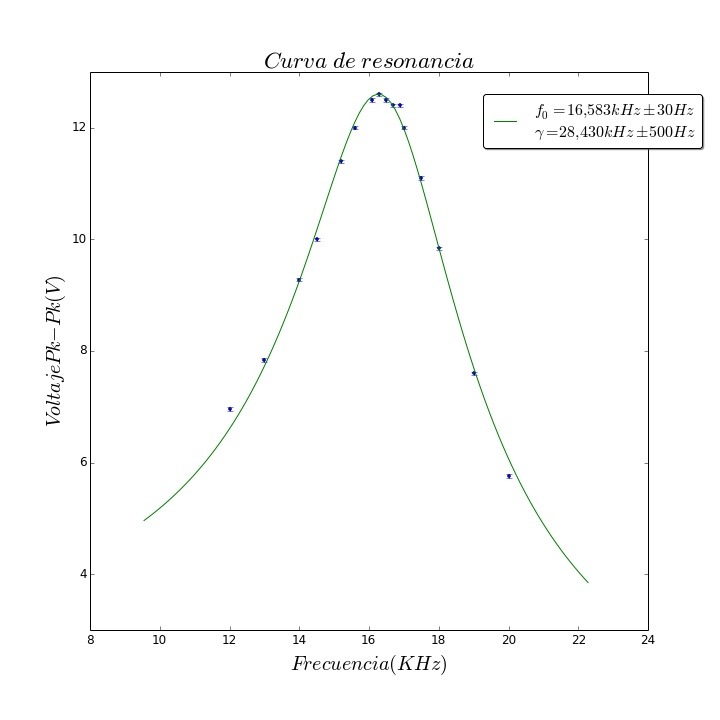
\includegraphics[width=0.45\textwidth]{resonancia}
\label{fig:resonancia}
\end{figure}

En esta gráfica se puede ver que el ajuste fue bastante preciso. Para verificarlo, tomamos el valor real de frecuencia angular natural $\omega_0^{Teo} = \frac{1}{2\pi \sqrt{LC}} = 16,416kHz$ y lo comparamos con el valor experimental obtenido  $\omega_0^{Exp} = 16,583kHz$. Debido a que no teníamos el error teórico, no sabremos con exactitud si el valor experimental entra en el rango aceptado. A pesar de esto, podemos afirmar que el error absoluto asociado a esta medición es del $1\%$.\\

De la misma manera podemos calcular experimentalmente el valor del t\'ermino $\gamma$ de resistencia. En teoría, dicho valor, teniendo en cuenta un\'icamente el valor de resistencia aportado por la inductancia, est\'a dado por $\gamma^{Teo} = \frac{R}{L} = 400Hz$; experimentalmente, esta cantidad tiene un valor de $\gamma^{Exp} = 28,430KHz$. Estos valores están desfasados por casi 2 \'ordenes de magnitud probablemente por no tener en cuenta todos los valores de resistencia asociados a los dem\'as aparatos usados.\\

Adem\'as del m\'etodo anterior podemos confirmar esta medida calculando el ancho de banda de la curva de resonancia. Teniendo el ajuste de par\'ametros, tenemos la funci\'on en pr\'acticamente cualquier frecuencia deseada. Con esto es muy sencillo calcular num\'ericamente y con gran precisi\'on el m\'aximo real de la curva. Con este m\'aximo, que se encuentra en $16,270KHz$ (se encuentra antes de la frecuencia natural como es esperado) podemos calcular los el valor que se tiene que alcanzar para calcular el ancho de banda ($\frac{A_{max}}{\sqrt{2}}$). Una vez calculados los valores de frecuencia que lo cumplen, obtenemos su diferencia y eso nos da el ancho de banda. El valor experimental obtenido para el ancho de banda es en este caso $\gamma^{ExpBW} = 28,996KHz$, lo cual confirma nuestro resultado anterior y le da fuerza a nuestro argumento. Podr\'iamos obtener $\gamma$ otra vez comparando la frecuencia angular natural $\omega_0$ y la frecuencia que provoca el m\'aximo en la curva de resonancia, sin embargo, este m\'etodo ser\'ia redundancia del ancho de banda y del uso de par\'ametros ajustados.\\
 


 


\section{\label{sec:level1}Conclusiones}



\subsection{\label{sec:citeref}Citations and References}
A citation in text uses the command \verb+\cite{#1}+ or
\verb+\onlinecite{#1}+ and refers to an entry in the bibliography. 
An entry in the bibliography is a reference to another document.

\subsubsection{Citations}
Because REV\TeX\ uses the \verb+natbib+ package of Patrick Daly, 
the entire repertoire of commands in that package are available for your document;
see the \verb+natbib+ documentation for further details. Please note that
REV\TeX\ requires version 8.31a or later of \verb+natbib+.

\paragraph{Syntax}
The argument of \verb+\cite+ may be a single \emph{key}, 
or may consist of a comma-separated list of keys.
The citation \emph{key} may contain 
letters, numbers, the dash (-) character, or the period (.) character. 
New with natbib 8.3 is an extension to the syntax that allows for 
a star (*) form and two optional arguments on the citation key itself.
The syntax of the \verb+\cite+ command is thus (informally stated)
\begin{quotation}\flushleft\leftskip1em
\verb+\cite+ \verb+{+ \emph{key} \verb+}+, or\\
\verb+\cite+ \verb+{+ \emph{optarg+key} \verb+}+, or\\
\verb+\cite+ \verb+{+ \emph{optarg+key} \verb+,+ \emph{optarg+key}\ldots \verb+}+,
\end{quotation}\noindent
where \emph{optarg+key} signifies 
\begin{quotation}\flushleft\leftskip1em
\emph{key}, or\\
\texttt{*}\emph{key}, or\\
\texttt{[}\emph{pre}\texttt{]}\emph{key}, or\\
\texttt{[}\emph{pre}\texttt{]}\texttt{[}\emph{post}\texttt{]}\emph{key}, or even\\
\texttt{*}\texttt{[}\emph{pre}\texttt{]}\texttt{[}\emph{post}\texttt{]}\emph{key}.
\end{quotation}\noindent
where \emph{pre} and \emph{post} is whatever text you wish to place 
at the beginning and end, respectively, of the bibliographic reference
(see Ref.~[\onlinecite{witten2001}] and the two under Ref.~[\onlinecite{feyn54}]).
(Keep in mind that no automatic space or punctuation is applied.)
It is highly recommended that you put the entire \emph{pre} or \emph{post} portion 
within its own set of braces, for example: 
\verb+\cite+ \verb+{+ \texttt{[} \verb+{+\emph{text}\verb+}+\texttt{]}\emph{key}\verb+}+.
The extra set of braces will keep \LaTeX\ out of trouble if your \emph{text} contains the comma (,) character.

The star (*) modifier to the \emph{key} signifies that the reference is to be 
merged with the previous reference into a single bibliographic entry, 
a common idiom in APS and AIP articles (see below, Ref.~[\onlinecite{epr}]). 
When references are merged in this way, they are separated by a semicolon instead of 
the period (full stop) that would otherwise appear.

\paragraph{Eliding repeated information}
When a reference is merged, some of its fields may be elided: for example, 
when the author matches that of the previous reference, it is omitted. 
If both author and journal match, both are omitted.
If the journal matches, but the author does not, the journal is replaced by \emph{ibid.},
as exemplified by Ref.~[\onlinecite{epr}]. 
These rules embody common editorial practice in APS and AIP journals and will only
be in effect if the markup features of the APS and AIP Bib\TeX\ styles is employed.

\paragraph{The options of the cite command itself}
Please note that optional arguments to the \emph{key} change the reference in the bibliography, 
not the citation in the body of the document. 
For the latter, use the optional arguments of the \verb+\cite+ command itself:
\verb+\cite+ \texttt{*}\allowbreak
\texttt{[}\emph{pre-cite}\texttt{]}\allowbreak
\texttt{[}\emph{post-cite}\texttt{]}\allowbreak
\verb+{+\emph{key-list}\verb+}+.

\end{document}
%
% ****** End of file apssamp.tex ******
